\documentclass{beamer}
\usepackage[utf8]{inputenc}
\usepackage[labelformat = empty, labelsep = none]{caption}
\usepackage{hyperref}

\usetheme{Madrid}
\usecolortheme{beaver}
\hypersetup{colorlinks=true, linkcolor=blue, filecolor=magenta, urlcolor=cyan}
\urlstyle{same}

\title{Amateur Telescope Making}
\subtitle{...or how to make your own telescope at home}
\author{Nuno Miguel Sousa}
\institute{Coimbra, Portugal}
\date{\today}


\begin{document}

\begin{frame}
\titlepage
\end{frame}

\begin{frame}
\frametitle{What is Amateur Telescope Making?}
\begin{block}{}
Amateur Telescope Making, or ATM, is a hobby taken by people that have an interest in astronomic observation and enjoy building telescopes.\footnotemark
\end{block}
\footnotetext{\url{https://en.wikipedia.org/wiki/Amateur_telescope_making}}
\begin{block}{}
ATM can range from just assembling the individually bought components to actually fabricate some or all of the components of a telescope.
\end{block}
\begin{block}{}
The most common type of telescope made by hobbyists is the so called Newtonian reflector (invented by Sir Isaac Newton).\footnotemark
\end{block}
\footnotetext{\url{https://en.wikipedia.org/wiki/Newtonian_telescope}}
\end{frame}

\begin{frame}
\frametitle{My personal motivation for ATM}
\begin{columns}
\column{0.6\textwidth}
One time by chance a few years ago, I had the opportunity to look up at the night sky in Alentejo's countryside, in southern Portugal.

The combination of very low light pollution and clear sky provided for a very distinctive view of the Milky Way.

I had some interest in astronomy in general, but that event was what sparked the beggining of my interest in astronomical observation.

Eventualy I found about ATM and ended up deciding to build a telescope myself because I found the challenge interesting.
\column{0.4\textwidth}
\begin{figure}
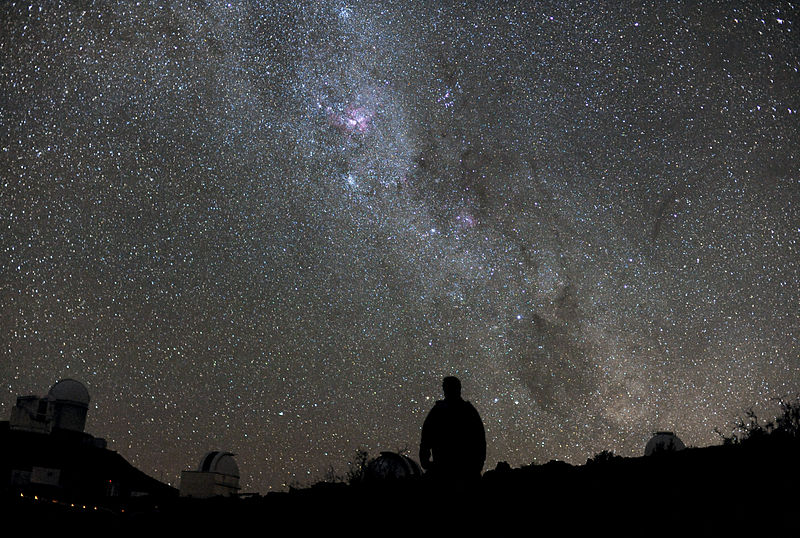
\includegraphics[scale=0.45]{assets/800px-Starry_Night_at_La_Silla.jpg}
\caption{Not me!}
\end{figure}
\end{columns}
\end{frame}

\begin{frame}
\frametitle{What I'm working on?}
I'm building a Newtonian reflector telescope and I'm making the main mirror lens myself.

It has a 200mm diameter main mirror and initially I planned for a focal length of 1200mm.

Why these characteristics?
\begin{itemize}
\item For a certain telescope diameter (aperture), it is the least complicated to make (only one convex main mirror lens and a small diagonal flat mirror).
\item A 200mm main mirror with 1200mm focal lenght is one of the most common configurations. It is a compromise between portability and light collection capability.
\item Provided you make some simple tools, the mirror's optical quality will only be limited by the amount of time you want to spend and pacience (or lack thereof).
\end{itemize}
\end{frame}

\begin{frame}
\frametitle{The Newtonian Reflector telescope}
\begin{figure}
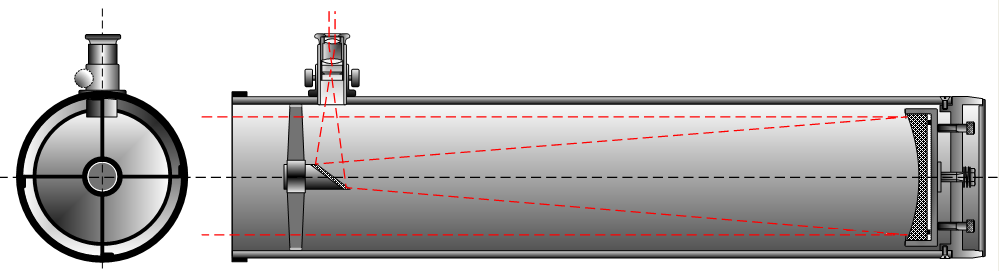
\includegraphics[scale=0.4]{assets/Newtontelescope.png}
\caption{Newtonian telescope}
\end{figure}
The main components of a Newtonian reflector telescope are the main concave mirror\footnotemark,\footnotetext{\url{https://en.wikipedia.org/wiki/Primary_mirror}}
the diagonal flat mirror, and the eyepiece\footnotemark.
\footnotetext{\url{https://en.wikipedia.org/wiki/Eyepiece}}

Incoming light (red dashed line) comes from the top of the telescope, iluminates the main mirror, and is reflected back to the eyepiece by the diagonal mirror.
\end{frame}

\begin{frame}
\frametitle{Making the main mirror}
For the main mirror you need a circular disc of some type of glass with a concave face on it.

Simple, right?

For an acceptale mirror, you will need a parabolic shaped surface that needs to have at most $0.15 \mu m$ of deviation from the theoretical ideal surface.

How do you make such an imposible smooth surface? By hand, of course.

\end{frame}

\begin{frame}
\frametitle{About the author}
My name is Nuno and ...
\end{frame}

\begin{frame}
\frametitle{The end}
Thank you!
\end{frame}

\end{document}
